\documentclass[11pt]{article}
\usepackage{geometry}
\usepackage{graphicx}
\usepackage{enumitem}
\usepackage{float}
\usepackage{amsmath}

\geometry{a4paper, top=0.5in, bottom=0.5in, right=0.75in, left=0.75in}

\title{DFT}
\author{Abanoub Emad Hanna}
\date{}

\begin{document}

\maketitle

\section*{Introduction}
Design for test is the act of adding additional hardware to ensure that the chip is working correctly after manufacturing. The challenge comes from absence of direct controllability and observability of the internal nodes of the chip. The nearer the gate to the primary input, the easier it is to control but difficult to observe, and vice versa.

\section*{Definitions}

\begin{minipage}{0.5\linewidth}
    \begin{itemize}
        \item \textbf{Testing:} Done on every finished chip.
        \item \textbf{Verification:}: Done on a design before fabrication.
        \item \textbf{Defect:} A physical problem that happened during fabrication.
        \item \textbf{Fault:} Modeling the \textbf{effect} (behaviour) of a defect (not necessarily the actual defect)  at a certain level of abstraction.
        \item \textbf{Error:} Wrong output due to a fault.
    \end{itemize}
\end{minipage}
\hfill
\begin{minipage}{0.45\linewidth}
    \begin{center}
        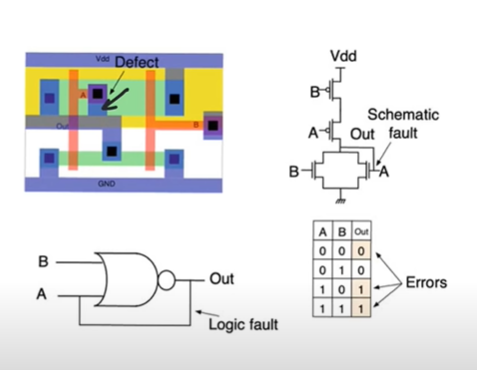
\includegraphics[scale=0.7]{1.png}
    \end{center}
\end{minipage}


\section*{Fault Coverage}
\begin{minipage}{0.5\linewidth}
    \begin{itemize}
        \item If we have M-bit input and N flip-flops (states), number of tests = $2^{M+N}$, which is impractical.
        \item Fault Coverage is the ratio between detected faults and total faults ($F=\frac{\text{detected faults}}{\text{total faults}}$).
        \item Fault coverage increases rapidly for a small number of tests, and then it starts to saturate slowly.
        \item Therefore, we carry out this small number of tests and tolerate the rest of the faults. 
    \end{itemize}
\end{minipage}
\hfill
\begin{minipage}{0.45\linewidth}
    \begin{center}
        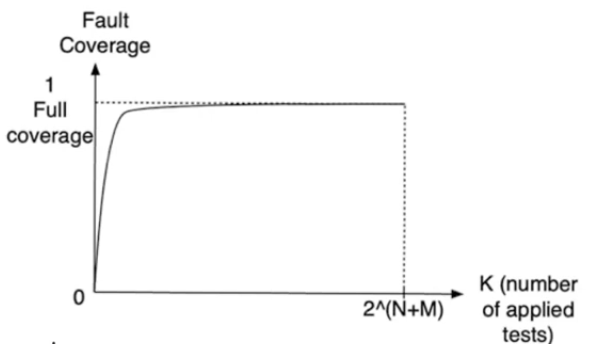
\includegraphics[scale=0.35]{2.png}
    \end{center}
\end{minipage}

\section*{Logic Testing}

\subsection*{Stuck-at Faults}
\begin{itemize}
    \item This models faults at the gate level.
    \item Any node could be either stuck-at-0 or stuck-at-1, so we have 2 possible faults per node. Total possible faults = $2*{N_{\text{gate nodes}}}$.
    \item We assume that only one fault occurs at a time (most likely scenario).
    \item We fill a truth table assuming that the fault is at a certain node, and then we compare it with the original thruth table to generate a test vector.
    \item Test vector is the smallest number of inputs that need to be applied to detect all possible faults.
    \item T=\{00,10,01\} for the following example.
\end{itemize}
\begin{center}
    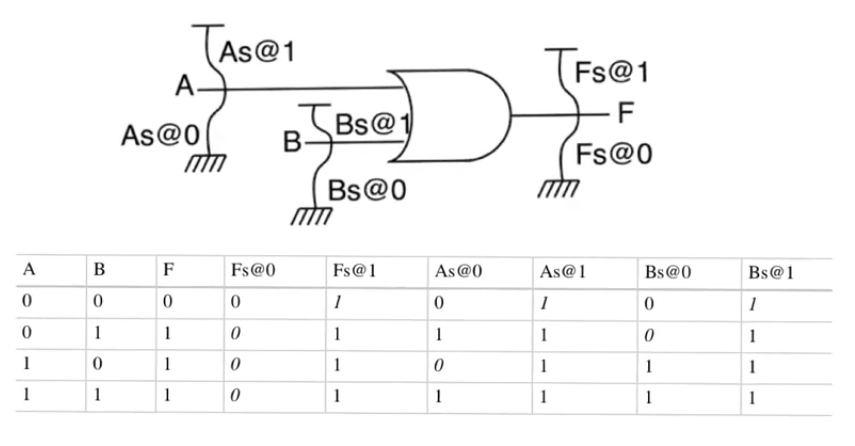
\includegraphics[width=0.65\textwidth]{3.png}
\end{center}

\subsection*{Stuck-Open/Short Faults}
\begin{itemize}
    \item This models faults at the transistor level.
    \item Any transistor could be either stuck-open or stuck-short, so we have 2 possible faults per transistor. Total possible faults = $2*{N_{\text{transistors}}}$.
    \item We assume that only one fault occurs at a time (most likely scenario).
    \item In order to detect a high impedance output (Z), we need to apply 2 inputs in sequence. 
    \item For example, for M1s0, we have to apply input to drive the output to $V_{DD}$ and then apply the input causing the high impedance. If output remains high, then the fault is detected.
\end{itemize}
\begin{center}
    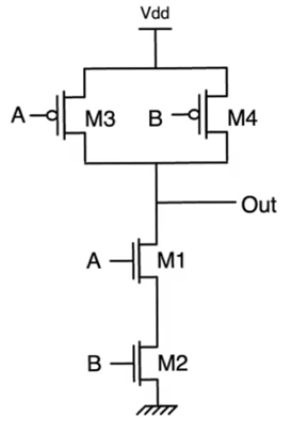
\includegraphics[width=0.25\textwidth]{4.png}
    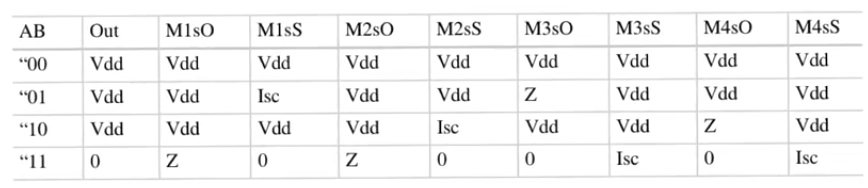
\includegraphics[width=0.65\textwidth]{5.png}
\end{center}

\subsection*{Scan Registers}
\begin{itemize}
    \item Replace every single pipeline register on the design with a scan register.
    \item SE: Scan Enable, this is the control signal that represents mode of operation (normal/scan).
    \item SI: Scan In, first register in the chain gets its input from an external pin. Other registers get their input from the previous register's SO: Scan Out.
    \item Last register's SO is connected to external pin.
    \item Note that the SO connection in the scan FF is actualy Q.
\end{itemize}

\begin{minipage}{0.55\textwidth}
    \subsubsection*{Effects}
    \begin{itemize}
      \item \textbf{Timing Overhead:}
        \begin{itemize}
          \item Higher setup time due to mux delay (try KVL method also).
          \item Higher clock-to-Q delay due to additional load from next scan FF.
        \end{itemize}
      \item \textbf{Area Overhead:} Additional area of the muxes.
    \end{itemize}    
\end{minipage}
\hfill
\begin{minipage}{0.35\textwidth}
  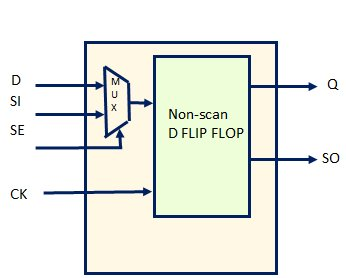
\includegraphics[scale=0.4]{1.jpg}
\end{minipage}

\subsection*{Operation}
\begin{enumerate}
    \item \textbf{Shift In:}
        \begin{itemize}
            \item SE is asserted, so that the scan FFs are connected like a shift register.
            \item We start shifting the test vector to store desired test case in the desired FF.
        \end{itemize}
    \item \textbf{Capture:}
        \begin{itemize}
            \item SE is de-asserted for 1 clock cycle so that the combinational logic provide an output.
        \end{itemize}
    \item \textbf{Shift Out:}
        \begin{itemize}
            \item SE is asserted again, and the value stored in the capture flop is shifted to the last FF to be obsereved at output pin.
        \end{itemize}
\end{enumerate}
\textbf{Note:} The disadvantage here is the deeper the pipeline, the higher the latency as you have to wait for input to be shifted in and the output to be shifted out.

\subsection*{Guidelines}
\begin{itemize}
    \item All the scan inputs in the scan FF should be controlled by the ATPG tool.
    \item All primary input clocks, generated clocks (e.g clock dividers) and resets should be muxed with a scan clock and scan reset respectively (scan mode is usually run on a slower clock to avoid any timing violations). MUX selector is test mode signal.
    \item Gated clocks are not controllable and should be bypassed in test mode.
    \item Do not replace shift registers with scan registers, just ensure the enable control.
\end{itemize}

\section*{Built-In Self-Test (BIST)}
\begin{center}
    \begin{minipage}{0.45\linewidth}
        \centering
        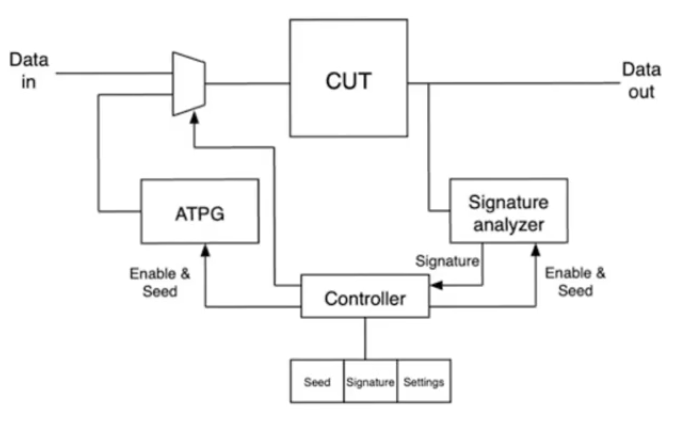
\includegraphics[width=1\linewidth]{6.png}
    \end{minipage}
    \hfill
    \begin{minipage}{0.45\linewidth}
        \centering
        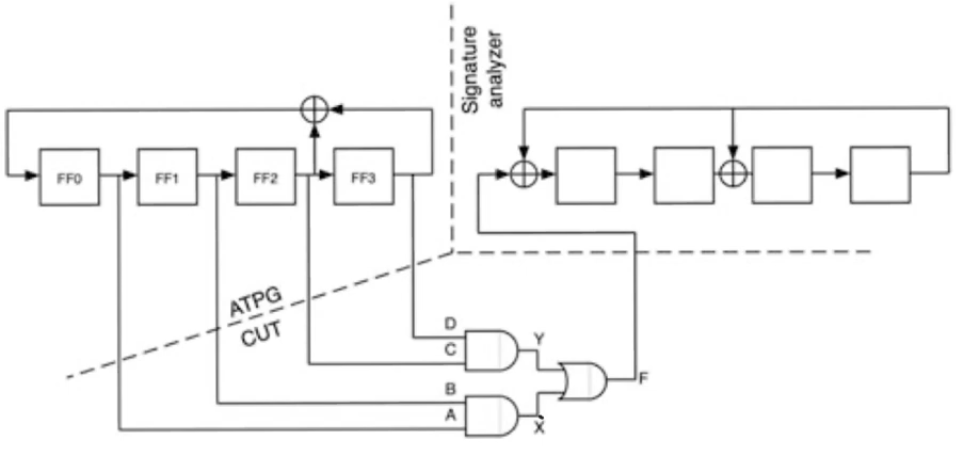
\includegraphics[width=1\linewidth]{7.png}
    \end{minipage}   
\end{center}
Now we consider a setup where the test is performed within the chip itself (BIST); one of the most well known forms of BIST is Power on Self Test (POST).
\begin{itemize}
    \item When the test signal is active, the input to the CUT (Circuit Under Test) is from the ATPG, and its output is given to a signature analyzer.
    \item Signature analyzer takes the outputs and automatically checks if the outputs fit with the correct outputs or not.
\end{itemize}
\subsection*{ATPG}
\begin{itemize}
    \item As discussed in fault coverage it's hard to cover all faults, so we should apply tests that combine the input bits in a random fashion so that it exposes as many faults as possible.
    \item On the other hand, the pattern applied cannot be truly random because we need to know the pattern to generate the gold standard against to compare the output.
    \item The sequence is pseudo-random noise (PN) sequence which is generated using linear feedback shift register (LSFR).
    \item The pattern of the LFSR has no input and generates a periodic sequence every $2^m - 1$ cycles based on an initial seed.
    \item The pattern itself can be concluded by knowing the initial pattern and the number of applied clock signal, but the bit change is random.
\end{itemize}

\begin{center}
    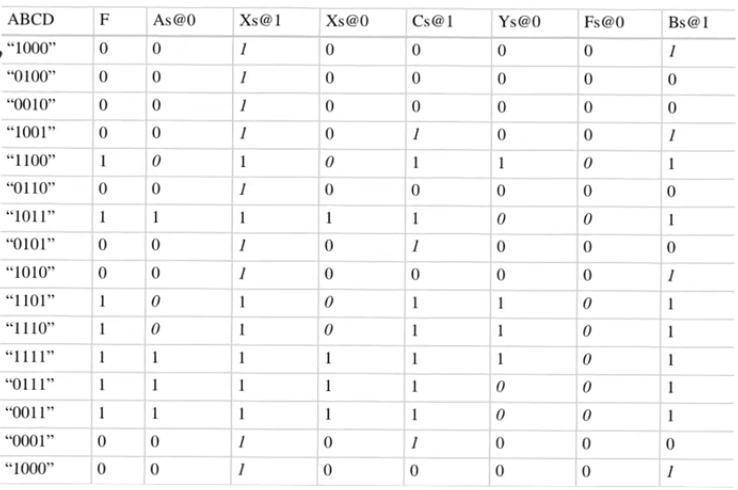
\includegraphics[width=0.6\textwidth]{8.png}
\end{center}

\subsection*{Signature Analyzer}
\begin{itemize}
    \item Testing all possible faults would require $2^{m}$ bit subtractors, which is impractical.
    \item The signature anayzer is similar to LFSR but has an external input and can have linear operations (XORs) between the registers of the shift register.
    \item The analyzer compresses the output sequence of CUT ($2^m$) into an n-bit signature that can specify the fault occured.
    \item Sequence of operation:
        \begin{enumerate}
            \item Initial seed is loaded to the registers (from designer).
            \item The output of the CUT (F) is fed to the signature analyzer.
            \item At the end of $2^m$ cycles, the contents of the register is the signature.
            \item Compare the signature with the golden signature (1000 in this example).
        \end{enumerate}
    \item However, the compressed signature may not be unique, so there is a trade-off between the number of bits (size of analyzer) and the uniqueness of the signature.
\end{itemize}
\begin{center}
    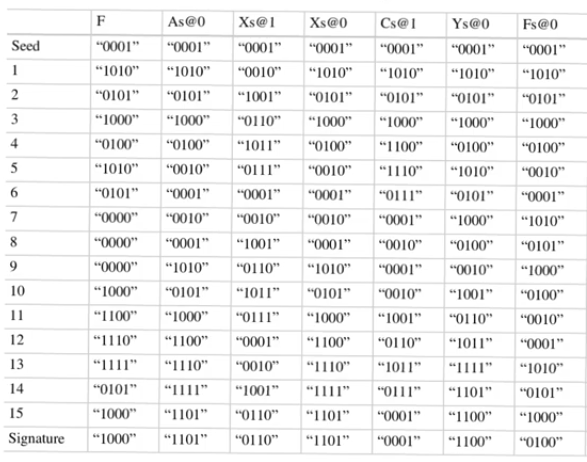
\includegraphics[width=0.6\textwidth]{9.png}
\end{center}

\section*{Memory Testing}

Memory March is a testing approach where we test a specific cell in the memory and we march to the next address until we reach the end of the memory. The high density of memories makes each cell affect the other and can't be tested in isolation.

\subsection*{Stuck-at Faults}
\begin{itemize}
    \item A zero is applied and read, then a one is applied and read.
    \item If the output is not the same as the input, then the cell is stuck at 0 or 1.
\end{itemize}

\subsection*{Transition Faults}
\begin{itemize}
    \item The cell can store a 0 or a 1, but it has a fault in the transition from 0 to 1 or from 1 to 0.
    \item \textbf{1-to-0 Transition:} Write 1, write 0, read 0.
    \item \textbf{0-to-1 Transition:} Write 0, write 1, read 1.
\end{itemize}

\subsection*{Coupling Faults}
Faults that occur due to the high density of the memory cells, where the fault involves two cells.
\subsubsection*{Briding Faults}
\begin{itemize}
    \item Two cells are bridged (shorted) to each other (bidirectional).
    \item If you change one the other changes too.
\end{itemize}

\subsubsection*{Inversion Faults}
\begin{itemize}
    \item Directional fault (the effect goes only in one direction); one cell has an impact on the other but not vice versa.
    \item a transition in one cell causes the other cell to invert its stored value.
\end{itemize}

\subsection*{Idempotent Faults}
\begin{itemize}
    \item It is a directional fault, where a transition in one cell sets a value in the other cell regardless of its previous value.
\end{itemize}

\subsection*{Coupling Faults Testing}
Idempotent fault (0 to 1 A transition sets B to 0) example:
\begin{itemize}
    \item Initialize A to 0 and B to 1.
    \item Write 1 to A and read B.
    \item If 1 is read, then this specific fault isn't present.
    \item If 0 is read, then we have to check if the fault is idempotent or inversion.
    \item Write 0 to both A and B.
    \item Write 1 to A and read B.
    \item If 0 is read, then this specific idempotent fault is present.
    \item If 1 is read, then this is an inversion fault.
\end{itemize}

\section*{NPSF (Neighbor Pattern Specific Fault)}
It is the most common fault and most difficult to detect. The fault here involves all neighboring cells (8 cells in 2D) affecting the central cell to have any fault from the stated before. 

\subsection*{Passive}
The presence of a specific pattern in all 8 neighboring cells, causes an erroneous behavior in the central cell.

\subsection*{Active}
Occurs when a pattern in the neighboring cells and a transition in one of them causes erroneous behavior in the central cell.

\end{document}